% !Mode:: "TeX:UTF-8"
%此为章节二模板
%\chapter、\section、\subsection、\subsubsection分别对应一二三四级标题
\chapter{图片示例}\label{ch:2}

\section{图片排版示例}
\textbf{注意}:使用 \verb|\caption[]{}| 命令时,如果不需要设置缩写目录的内容,一定要删掉[],否则插图插表索引将不会显示该图或表的目录。

\textbf{建议}:在论文写作时图片位置可以先按照写作时的习惯进行放置,待到完成所有写作内容后再进行详细调整图片位置。

\subsection{图片格式}

\LaTeX 中图片推荐使用pdf格式。使用Origin可导出矢量无白边的图片以保证清晰度,其次推荐使用jpg,png格式图片。

为了保证图片的清晰,jpg图片导出时ppi建议设置为300,png图片导出时建议宽度设置为1024像素(可根据需求自行设置),长度随宽度变化。

\subsection{单图排版示例}

\begin{figure}[htb]
    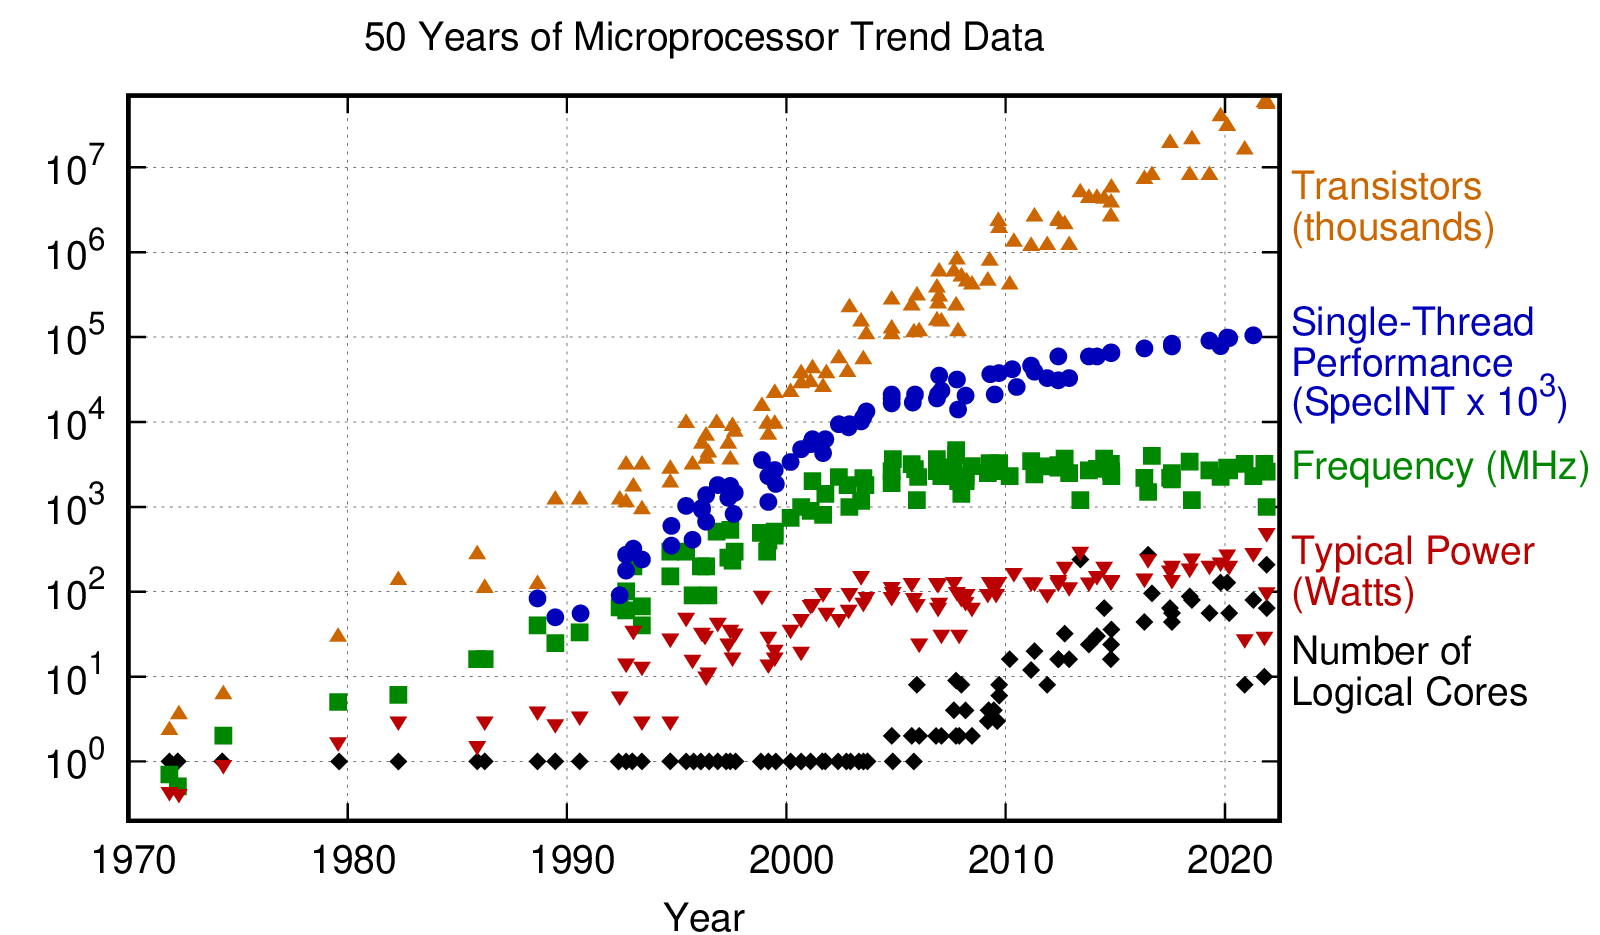
\includegraphics[width=0.8 \textwidth]{50-years-processor-trend.png}
    \caption[处理器发展]{近50年微处理器发展趋势} % 中括号中内容为插图索引中显示内容,可在题注内容过长时使用
    \label{fig:processor-trend}
\end{figure}

图片引用示例:\cref{fig:processor-trend}。

\subsection{多图排版示例}
同一行中的子图之间要留有空间,不要占满!否则会自动换行!

子图之间空一行表示换行。

插入子图请使用 \verb|\subfloat{}| 命令。

\begin{figure}[htb]
    \subfloat[改进前的结构]{
        \label{fig:Unimproved-cooling-structure}
        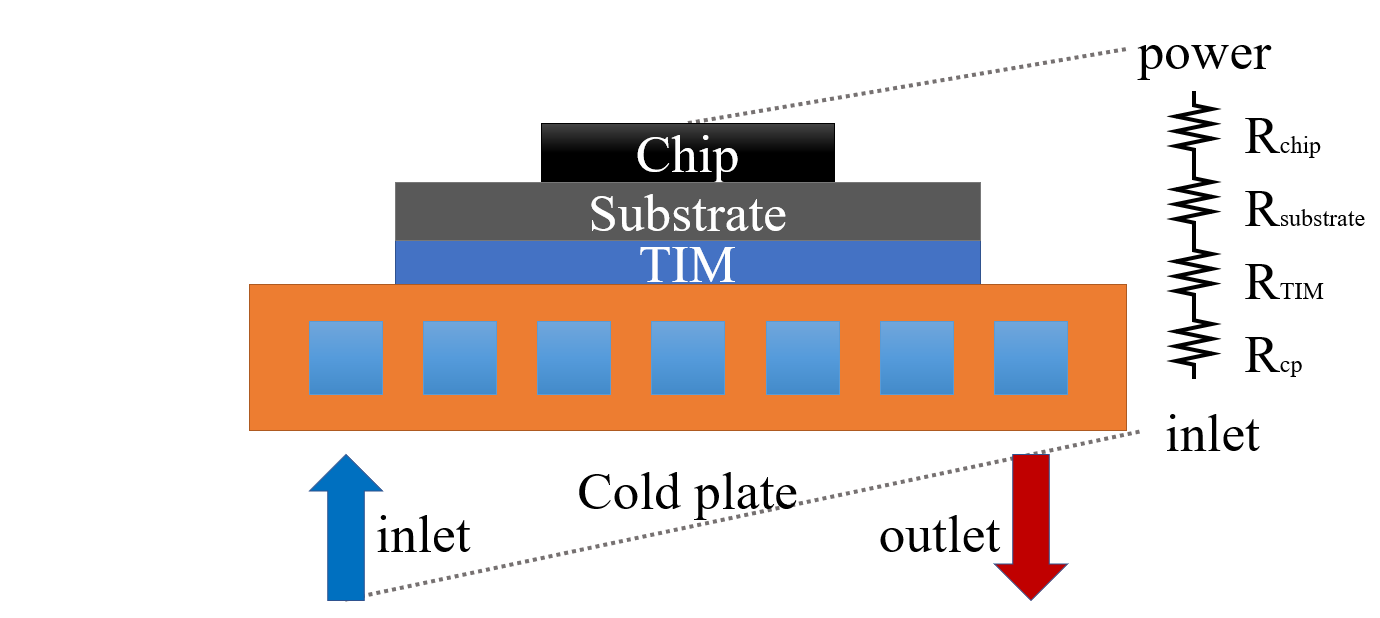
\includegraphics[width=0.45\linewidth]{Unimproved-cooling-structure.png}}
    \subfloat[基板内进行微通道散热]{
        \label{fig:LTCC-Microchannels}
        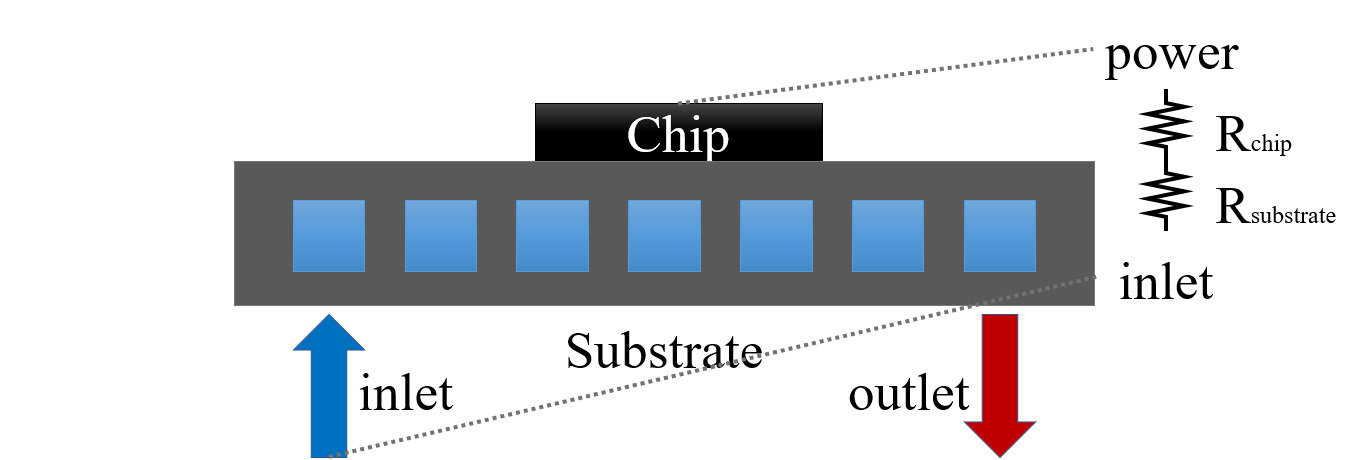
\includegraphics[width=0.45\linewidth]{LTCC-Microchannels.png}}

    \subfloat[嵌入散热模块]{
        \label{fig:Embedded-cooling-module}
        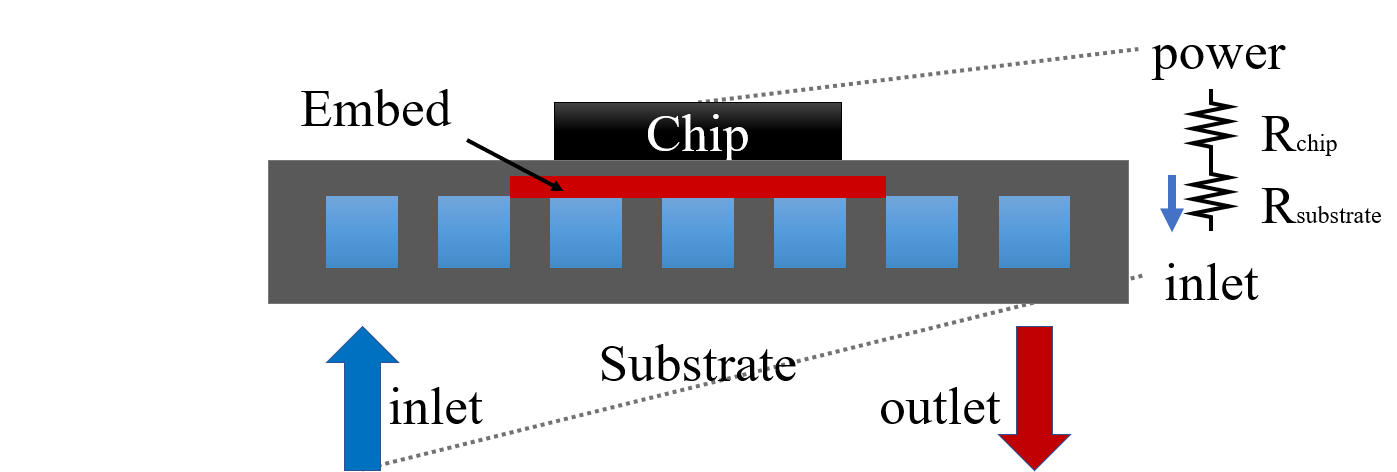
\includegraphics[width=0.45\linewidth]{Embedded-cooling-module.png}}
    \subfloat[带针鳍或肋的嵌入式散热模块]{
        \label{fig:Rib-pin-fin}
        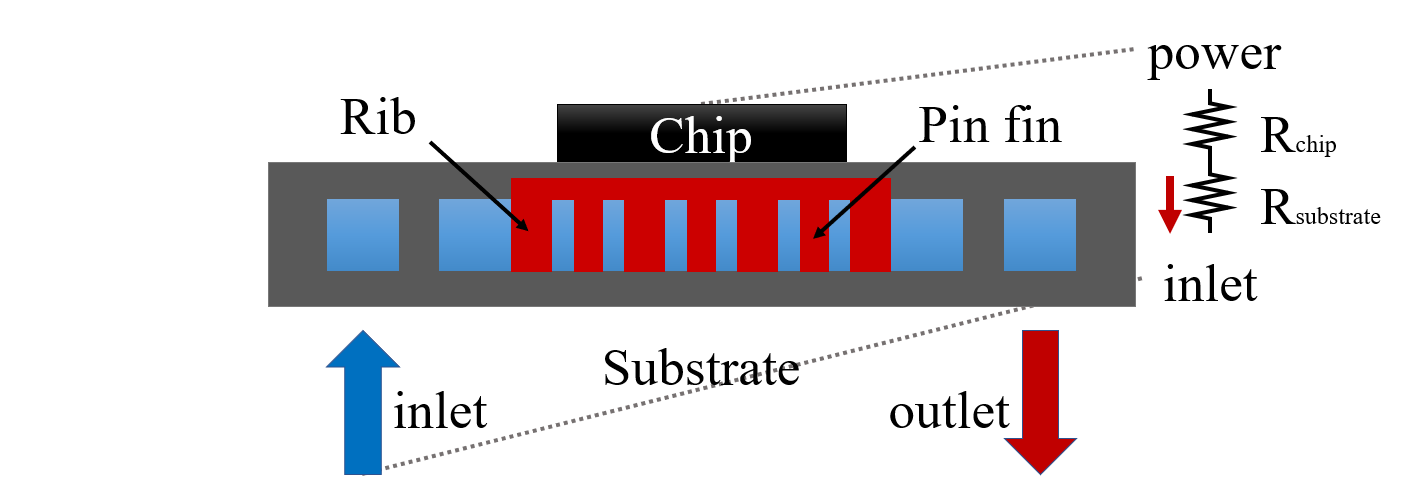
\includegraphics[width=0.45\linewidth]{Rib-pin-fin.png}}
    \caption{三种强化传热途径示意图}
    \label{fig:Three-enhanced-heat-transfer-paths}
\end{figure}

子图引用示例:\cref{fig:Unimproved-cooling-structure},

整图引用示例:\cref{fig:Three-enhanced-heat-transfer-paths}。

提供三种不同的Tikz绘图示例,分别为柱状图(第一个子图存在问题是少一列,是由于间距放不下导致的,可以参考第二张图进行对应的修改),多点折线图,少点折线图。

\begin{figure}
    \subfloat[生成证明\label{fig-2}]{
        \begin{tikzpicture}[global scale = 0.55]
            \begin{axis}[
                x tick label style={
                    /pgf/number format/1000 sep=.},
                y tick label style={
                    /pgf/number format/1000 sep=.},
                xlabel={参与者数量},            % x轴标题
                ylabel={耗时 (ms)},             % y轴标题
                ymin=0, ymax=1100,              % y轴范围
                ybar=10pt,                      % 柱状图间距
                bar width=20pt,                 % 柱状图宽度
                enlarge x limits={abs=6pt},     % x轴左右空白
                legend cell align={left},       % 图例位置
                enlarge y limits={value=0.1,upper}, % y轴上下空白
                ybar interval=0.7,                  % 柱状图间距
                legend pos=north west,              % 图例位置
                xtick=data,                         % x轴数据
                xticklabels={100, 200, 300, 400, 500},  % x轴标签
                ytick={0, 500, 1000},                   % y轴标签
                legend style={font=\huge},              % 图例字体大小
                label style={font=\huge},               % 标签字体大小
                tick label style={font=\huge}           % 刻度字体大小    
                ]
                \addplot[color=orange,fill=orange!50,bar shift=-6pt] coordinates {
                    (1,216.7)
                    (2,434.6)
                    (3,512.1)
                    (4,637.2)
                    (5,751.4)
                };
                \addplot[color=blue,fill=blue!50,bar shift=-2pt] coordinates {
                    (1,314.3)
                    (2,251.5)
                    (3,428.7)
                    (4,835.9)
                    (5,1203.1)
                };
                \addplot[color=green,fill=green!50,bar shift=0pt] coordinates {
                    (1,705.824)
                    (2,103.074)
                    (3,270.234)
                    (4,1067.464)
                    (5,1024.614)
                };
                \addplot[color=gray,fill=gray!50,bar shift=2pt] coordinates {
                    (1,130.214)
                    (2,261.854)
                    (3,393.414)
                    (4,525.034)
                    (5,656.674)
                };
                \addplot[color=red,fill=red!50,bar shift=6pt] coordinates {
                    (1,117.529)
                    (2,336.439)
                    (3,743.239)
                    (4,870.919)
                    (5,988.179)
                };
                \legend{XXX et al.\cite{Lau_2022},YYY et al.\cite{Lau_2022},ZZZ et al.\cite{Lau_2022},HHH et al.\cite{Lau_2022},本方案}
            \end{axis}
        \end{tikzpicture}
    }
    \hfill
    \subfloat[包括Soot的类加载持续时间在内的时间消耗比较\label{fig-3}]{
        \begin{tikzpicture}[global scale = 0.65]
            \begin{axis}[
                xlabel={样本名称},
                ylabel={时间 (毫秒)},
                symbolic x coords={A,B,C,D,E},
                xtick=data,             % x轴数据
                bar width=20pt,         % 柱状图宽度
                nodes near coords,      % 柱状图上显示数值
                ymin=0, ymax=48000,     % y轴范围
                ybar=10pt,              % 柱状图间距
                width=0.65\linewidth,   % 图片宽度
                bar width = 12pt,       % 柱状图宽度
                enlarge x limits={abs=30pt},    % x轴左右空白
                ylabel style={yshift=-10pt},    % y轴标题位置
                legend cell align={left},       % 图例位置
                enlarge y limits={value=0.1,upper}, % y轴上下空白
                legend pos=north west,              % 图例位置
                nodes near coords style={font=\Large}, % 柱状图上数值字体大小,不够的话自行调整
                legend style={font=\huge},              % 图例字体大小
                label style={font=\huge},               % 标签字体大小
                tick label style={font=\huge}           % 刻度字体大小
                ]
                \addplot[color=blue,fill=blue!50,bar shift=-9pt] coordinates {
                    (A,35248)
                    (B,36173 )
                    (C,14249)
                    (D,15963)
                    (E,12385 )
    
                };
                 \addlegendentry{Soot与数据流分析}
                \addplot[color=red,fill=red!50,bar shift=9pt] coordinates {
    
                    (A,2796)
                    (B,2885)
                    (C,1649)
                    (D,1193)
                    (E,537)
                };
                \addlegendentry{LightSim}
            \end{axis}
        \end{tikzpicture}
    }
    \caption{示例图}
    \label{fig3}
\end{figure}

在\cref{fig-2}和\cref{fig-3}中,是引用。

\begin{figure}[tbh!]
    \subfloat[MNIST\label{fig-4}]{
        \begin{tikzpicture}[global scale = 0.6]
            \begin{axis}[
                xlabel={迭代次数},
                ylabel={准确率 (\%)},
                xticklabel style={anchor= east,rotate=45 },
                xmax=250,
                xmin=0,
                ymax=100,
                ymin=38,
                legend pos=south east,
                ymajorgrids=true,
                grid style=dashed,
                legend style={nodes={scale=1, transform shape}},
                legend style={font=\huge},
                label style={font=\huge},
                tick label style={font=\huge}
                ]
                \addplot[
                color=blue,
                mark=.,
                only marks,
                sharp plot,
                line width=1.5pt
                ] table [x index=0, y index=1] {Data/data_sub_2.dat};
                \addplot[
                color=green,
                mark=.,
                only marks,
                sharp plot,
                line width=1.5pt
                ] table [x index=0, y index=2] {Data/data_sub_2.dat};
                \addplot[
                color=red,
                mark=.,
                only marks,
                sharp plot,
                line width=1.5pt
                ] table [x index=0, y index=3] {Data/data_sub_2.dat};
                \legend{100 参与者, 300 参与者, 500 参与者}
            \end{axis}
        \end{tikzpicture}
    }
    \hfill
    \subfloat[CIFSAR{\footnotesize 100}\label{fig-5}]{
        \begin{tikzpicture}[global scale = 0.6]
            \begin{axis}[
                xlabel={迭代次数},
                ylabel={准确率 (\%)},
                xticklabel style={anchor= east,rotate=45 },
                xmax=250,
                xmin=0,
                ymax=80,
                ymin=23,
                legend pos=south east,
                ymajorgrids=true,
                grid style=dashed,
                legend style={nodes={scale=1, transform shape}},
                legend style={font=\huge},
                label style={font=\huge},
                tick label style={font=\huge}
                ]
                \addplot[
                color=blue,
                mark=.,
                only marks,
                sharp plot,
                line width=1.5pt
                ] table [x index=0, y index=1] {Data/data_sub_1.dat};
                \addplot[
                color=green,
                mark=.,
                only marks,
                sharp plot,
                line width=1.5pt
                ] table [x index=0, y index=2] {Data/data_sub_1.dat};
                \addplot[
                color=red,
                mark=.,
                only marks,
                sharp plot,
                line width=1.5pt
                ] table [x index=0, y index=3] {Data/data_sub_1.dat};
                \legend{100 参与者, 300 参与者, 500 参与者}
            \end{axis}
        \end{tikzpicture}
    }
    \caption[方案一的准确度与迭代次数关系]{不同数量的客户端的准确性与迭代次数的关系}
    \label{exp1}
\end{figure}

\begin{figure}[tbh!]
    \subfloat[MNIST\label{fig-6}]{
        \begin{tikzpicture}[global scale = 0.6]
            \begin{axis}[
                xlabel={参与者数量},
                ylabel={准确率 (\%)},
                symbolic x coords = {100,200,300,400,500},
                xticklabel style={anchor= east,rotate=45 },
                xtick=data,
                ymax=100,
                ymin=40,
                legend pos=south east,
                legend cell align={left},
                ymajorgrids=true,
                grid style=dashed,
                legend style={nodes={scale=1, transform shape}},
                legend style={font=\huge},
                label style={font=\huge},
                tick label style={font=\huge}
                ]
                \addplot+[mark size=3pt]
                coordinates {
                    (100, 91.0349)
                    (200, 91.7635)
                    (300, 92.1530)
                    (400, 93.5713)
                    (500, 94.2747)
                };\label{6c0}
                \addplot+[mark size=3pt]
                coordinates {
                    (100, 88.4214)
                    (200, 88.6571)
                    (300, 89.5672)
                    (400, 90.6631)
                    (500, 91.2861)
                };\label{6c1}
                \addplot+[mark size=3pt]
                coordinates {
                    (100, 86.8072)
                    (200, 87.0289)
                    (300, 88.9112)
                    (400, 89.7785)
                    (500, 90.0550)
                };\label{6c2}
                \addplot+[mark size=3pt]
                coordinates {
                    (100, 90.5275)
                    (200, 90.1048)
                    (300, 91.8314)
                    (400, 92.4257)
                    (500, 93.5617)
                };\label{6c3}
                \addplot+[mark size=3pt]
                coordinates {
                    (100, 91.2241)
                    (200, 91.7189)
                    (300, 92.6760)
                    (400, 93.1523)
                    (500, 93.8426)
                };\label{6c4}
                \addplot+[mark size=3pt]
                coordinates {
                    (100, 86.4234)
                    (200, 88.3281)
                    (300, 89.5347)
                    (400, 90.2071)
                    (500, 91.8193)
                };\label{6c5}
                \addplot+[mark size=3pt]
                coordinates {
                    (100, 82.6479)
                    (200, 85.4558)
                    (300, 87.1009)
                    (400, 88.3564)
                    (500, 89.6152)
                };\label{6c6}
                \addplot+[mark size=3pt]
                coordinates {
                    (100, 73.4036)
                    (200, 76.6815)
                    (300, 77.5426)
                    (400, 78.1326)
                    (500, 78.9213)
                };\label{6c7}
            \legend{本方案, XXX et al.\cite{Lau_2022}, YYY et al.\cite{Lau_2022}, ZZZ et al.\cite{Lau_2022}, HHH et al.\cite{Lau_2022}, 5\% 恶意参与者, 10\% 恶意参与者, 20\% 恶意参与者}
            \end{axis}
        \end{tikzpicture}
    }
    \hfill
    \subfloat[CIFSAR{\footnotesize 100}\label{fig-7}]{
        \begin{tikzpicture}[global scale = 0.6]
            \begin{axis}[
                %title={},
                xlabel={参与者数量},
                ylabel={准确率 (\%)},
                symbolic x coords = {100,200,300,400,500},
                xticklabel style={anchor= east,rotate=45 },
                xtick=data,
                ymax=80,
                ymin=20,
                legend pos=south east,
                legend cell align={left},
                ymajorgrids=true,
                grid style=dashed,
                legend style={nodes={scale=1, transform shape}},
                legend style={font=\huge},
                label style={font=\huge},
                tick label style={font=\huge}
                ]
                \addplot+[mark size=3pt]
                coordinates {
                    (100, 73.0039)
                    (200, 73.4271)
                    (300, 73.7160)
                    (400, 74.2513)
                    (500, 75.0248)
                };
                \addplot+[mark size=3pt]
                coordinates {
                    (100, 70.5137)
                    (200, 71.2461)
                    (300, 71.5914)
                    (400, 72.6225)
                    (500, 73.3046)
                };
                \addplot+[mark size=3pt]
                coordinates {
                    (100, 70.0164)
                    (200, 71.2286)
                    (300, 72.1332)
                    (400, 72.4517)
                    (500, 73.1561)
                };
                \addplot+[mark size=3pt]
                coordinates {
                    (100, 72.3538)
                    (200, 72.6216)
                    (300, 73.8918)
                    (400, 74.2905)
                    (500, 74.1621)
                };
                \addplot+[mark size=3pt]
                coordinates {
                    (100, 72.1013)
                    (200, 73.5135)
                    (300, 73.9425)
                    (400, 74.7297)
                    (500, 75.2756)
                };
                \addplot+[mark size=3pt]
                coordinates {
                    (100, 68.5217)
                    (200, 70.4832)
                    (300, 71.7219)
                    (400, 72.0186)
                    (500, 72.3318)
                };
                \addplot+[mark size=3pt]
                coordinates {
                    (100, 62.2815)
                    (200, 65.8233)
                    (300, 67.6183)
                    (400, 68.1124)
                    (500, 69.5276)
                };
                \addplot+[mark size=3pt]
                coordinates {
                    (100, 53.6133)
                    (200, 55.5052)
                    (300, 58.4218)
                    (400, 61.1081)
                    (500, 62.3716)
                };
                \legend{本方案, XXX et al.\cite{Lau_2022}, YYY et al.\cite{Lau_2022}, ZZZ et al.\cite{Lau_2022}, HHH et al.\cite{Lau_2022}, 5\% 恶意参与者, 10\% 恶意参与者, 20\% 恶意参与者}
            \end{axis}
        \end{tikzpicture}
    }
    \caption[方案一的准确度比较]{准确度比较}
    \label{exp2}
\end{figure}

引用也是一样的,如\cref{fig-4}和\cref{fig-5}。和\cref{fig-6}和\cref{fig-7}。以及对整个图的引用\cref{exp1}和\cref{exp2}。

\section{本章小节}
本章介绍了基于嵌入式散热模块的微通道散热技术所涉及的基……